\chapter{VBO}
\begin{tabular}{lcccc}
			& Kartesische Koord. 	& Farben 		& Textur-Koord. & Normal			\\
	$v_0$	& $x_0, y_0,z_0,w_0 $	& $r_0,g_0,b_0$	& $s_0,t_0$		& $u_0, v_0, w'_0$	\\
	$v_1$	&						&				&				&					\\
	$\vdots$&						&				&				&					\\
	$v_{n-1}$&						&				&				&					
\end{tabular}\\
\begin{tabular}{ll}
	Entweder alles in einen Buffer &$\Rightarrow$ Array of Structs\\
	Oder für jede Klasse einen eigenen Buffer &$\Rightarrow$ Struct of Array % Sorum richtig? 
\end{tabular}
\begin{tikzpicture}
\end{tikzpicture}

\begin{figure}[H]
	\begin{subfigure}{.47\textwidth}
	\centering
	\begin{tikzpicture}
\begin{axis}[clip = false, axis lines = none, xmin = 0, xmax = 2, ymin=0, ymax=2, axis equal]
%\addplot {};
\draw[step=.1] (axis cs:0,0) grid (axis cs: 2,2);
\draw (axis cs:0,0) -- (axis cs:1.05,2) -- (axis cs:2,0.55) -- (axis cs:0,0);
%\draw[xstep = 10, ystep = 10, gray, very thin] (axis cs:0,0) grid (axis cs:2,2);
\node[anchor=north] at (axis cs:0,0) {$V_0$};
\node at (axis cs:0.45,0.45) (x) {x};
\node at ($(x) - (0,1)$) (t) {interpolierte Farbe z.B. Mischung};
\draw[-latex] (t)--(x);
\node[anchor=west] at (axis cs:2,0.55) {$V_1$};
\node[anchor=south] at (axis cs:1.05,2) {$V_2$};
\node[anchor=north] at (axis cs:0,-0.2) {r};
\node[anchor=west] at (axis cs:2.1,0.4) {g};
\node[anchor=south] at (axis cs:1.1,2.2) {b};
\end{axis}
\end{tikzpicture}
\caption{Beispiel Raster}
\end{subfigure}
\begin{subfigure}{.47\textwidth}
	\centering
	\begin{tikzpicture}
	\begin{axis}[clip = false, axis lines = none, xmin = 0, xmax = 2, ymin=0, ymax=2, axis equal]
	%\addplot {};
	\addplot[ patch, shader = interp, mesh/color input = explicit]
	coordinates {
		(0,0)[color=red] (1.05,2)[color=blue] (2,0.55)[color=green]};
	\draw[step=.1] (axis cs:0,0) grid (axis cs: 2,2);
	%\draw[xstep = 10, ystep = 10, gray, very thin] (axis cs:0,0) grid (axis cs:2,2);
	\node[anchor=north] at (axis cs:0,0) {$V_0$};
	\node[text=white] at (axis cs:0.45,0.45) (x) {x};
	\node at ($(x) - (0,1)$) (t) {interpolierte Farbe z.B. Mischung};
	\draw[-latex, decoration={color change, start color=black, end color = white}, decorate] (t)--(x);
	\node[anchor=west] at (axis cs:2,0.55) {$V_1$};
	\node[anchor=south] at (axis cs:1.05,2) {$V_2$};
	\node[anchor=north] at (axis cs:0,-0.2) {r};
	\node[anchor=west] at (axis cs:2.1,0.4) {g};
	\node[anchor=south] at (axis cs:1.1,2.2) {b};
	\end{axis}
	\end{tikzpicture}
	\caption{Beispiel Mischung der Farben}
\end{subfigure}

\end{figure}
Shader nimmt die Attribute von den Randpunkten und prozessiert diese auf die Pixel im inneren des Dreiecks.
\pagebreak
\section{Baryzentrische Koordinaten}
\fbox{varying} im Vertexshader
\begin{figure}[H]
	\centering
	\begin{tikzpicture}
\begin{axis}[clip = false, axis lines = none, xmin = 0, xmax = 2, ymin=0, ymax=2]
%\addplot {};
\draw (axis cs:0,0) -- (axis cs:1,2) -- (axis cs:2,0.5) -- (axis cs:0,0);
\node[anchor=north] at (axis cs:0,0) {a};
\node[anchor=west] at (axis cs:2,0.5) {b};
\node[anchor=south] at (axis cs:1,2) {c};
\node at (axis cs:0.5,0.5) {x};
\node[anchor=north] at (axis cs:0,-0.2) {f(a)};
\node[anchor=west] at (axis cs:2.1,0.4) {f(b)};
\node[anchor=south] at (axis cs:1.1,2.2) {f(c)};
\end{axis}
\end{tikzpicture}
\caption{Baryzentrisches Koordinatensystem}
\end{figure}
\[ \vektor{a_1&b_1&c_1\\a_2&b_2&c_2\\1&1&1} \cdot \dddvec{\alpha}{\beta}{\gamma} = \dddvec{x_1}{x_2}{1} \]
\[ x = \alpha\cdot a + \beta \cdot b + \gamma\cdot c \land  \alpha+\beta+\gamma = 1 \]
\[ \Rightarrow f(x) = \alpha\cdot f(a) + \beta\cdot f(b) + \gamma \cdot f(c) \]
\section{Texturen}
\subsection{Mipmap}
\begin{figure}[H]
\begin{tikzpicture}[scale=1]
\node[anchor=south] at (3.5,7) {$w$};
\node[anchor=west] at (7,3.5) {$h$};
\draw (0,0) rectangle (7,7);
\end{tikzpicture}
\begin{tikzpicture}[scale=1/2]
\node[anchor=south] at (3.5,7) {$\frac{w}{2}$};
\node[anchor=west] at (7,3.5) {$\frac{h}{2}$};
\draw (0,0) rectangle (7,7);
\end{tikzpicture}
\begin{tikzpicture}[scale=1/4]
\node[anchor=south] at (3.5,7) {$\frac{w}{4}$};
\node[anchor=west] at (7,3.5) {$\frac{h}{4}$};
\draw (0,0) rectangle (7,7);
\end{tikzpicture}
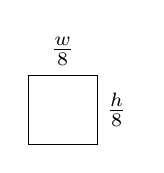
\begin{tikzpicture}[scale=1/8]
\node[anchor=south] at (3.5,7) {$\frac{w}{8}$};
\node[anchor=west] at (7,3.5) {$\frac{h}{8}$};
\draw (0,0) rectangle (7,7);
\end{tikzpicture}
\end{figure}

\[ S = \sum_{i=0}^{\infty} (\frac{1}{4})^i = \frac{1}{1 - \frac{1}{4}} = \frac{4}{3} \]

\pagebreak

\begin{figure}[H]
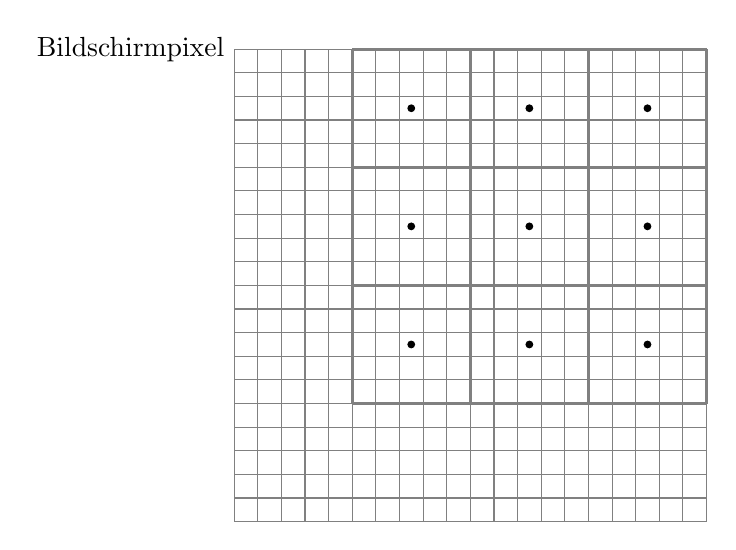
\begin{tikzpicture}[scale=3]
%\begin{axis}[clip = false, axis lines = none, ylabel={Bildschirmpixel}, xmin = 0, xmax=2, ymin = 0, ymax = 2]
\draw[step = .1, gray, thin] (0,0) grid (2,2);
\draw[step = .5, gray, very thick] (0.5,0.5) grid (2,2);
\node[anchor=east] at (0,2) {Bildschirmpixel};
\node[fill, circle, inner sep = 1] at (0.75,0.75) {};
\node[fill, circle, inner sep = 1] at (1.25,0.75) {};
\node[fill, circle, inner sep = 1] at (1.75,0.75) {};
\node[fill, circle, inner sep = 1] at (0.75,1.25) {};
\node[fill, circle, inner sep = 1] at (1.25,1.25) {};
\node[fill, circle, inner sep = 1] at (1.75,1.25) {};
\node[fill, circle, inner sep = 1] at (0.75,1.75) {};
\node[fill, circle, inner sep = 1] at (1.25,1.75) {};
\node[fill, circle, inner sep = 1] at (1.75,1.75) {};
%\end{axis}
\end{tikzpicture}
\end{figure}

\begin{figure}[H]
	\centering
	\begin{tikzpicture}[scale=3]
		\node[fill, circle, inner sep=1] at (0,0) (A) {};
		\node[fill, circle, inner sep=1] at (1,0) (B) {};
		\node[fill, circle, inner sep=1] at (0,1) (C) {};
		\node[fill, circle, inner sep=1] at (1,1) (D) {};
		\draw (A) -- (B);
		\draw (C) -- (D);
		\node[draw, circle, inner sep = 1] at (.2, 1) (E){};
		\node[draw, circle, inner sep = 1] at (.2, 0) (F){};
		\node[draw, inner sep = 2] at (.2, .2) {};
		\node[fill, circle, inner sep = .25] at (.2, .2) {};
		\draw (E) -- (F);
		\draw[dashed] (.5,-.2) -- (.5,1.2);
		\draw[dashed] (-.2,.5) -- (1.2,.5);
	\end{tikzpicture}
	\caption{bilineare Interpolation}
\end{figure}

\begin{figure}[H]
\begin{tikzpicture}[scale = 3]
\draw (0,0) rectangle (1,1);
\node[anchor=south east] at (0,1) {$(-1,1)$};
\node[anchor=south west] at (1,1) {$(1,1)$};
\node[anchor=north east] at (0,0) {$(x,y) = (-1,-1)$};
\node[anchor=north west] at (1,0) {$v_0~(1,-1)$};

\node[anchor=south east] at (0,1-0.175) {$(0,0)$};
\node[anchor=south west] at (1,1-0.175) {$(3,0)$};
\node[anchor=north east] at (0,0-0.175) {$(s_3, t_3) = (0,3)$};
\node[anchor=north west] at (1,0-0.175) {$(s_0,t_0) = (3,3) $};
\end{tikzpicture}
\end{figure}
In der Regel sind Texturkoordinaten in $[0,1]^2$, wenn größer wird sie periodisch verwendet.
\begin{figure}[H]
	\centering
	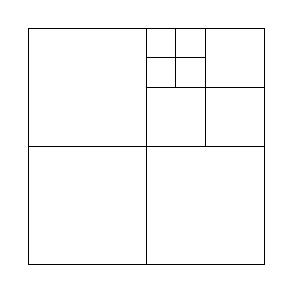
\begin{tikzpicture}[scale=3]
		\draw (0,0) rectangle (1,1);
		\draw[step=.5] (0,0) grid (1,1);
		\draw[step=.25] (.5,.5) grid (1,1);
		\draw[step=.125] (.5,.75) grid (.75,1);
	\end{tikzpicture}
	\caption{Maps Mipmapping}
\end{figure}